\section{Introduction}
\label{sec:intro:0}

The Vera C. Rubin Observatory’s Data Preview 1 (DP1) marks an important milestone in preparing for the forthcoming Legacy Survey of Space and Time (LSST), offering a valuable opportunity to test and validate scientific tools and workflows on precursor imaging data. Among the core scientific objectives of LSST is the estimation of photometric redshifts (photo-zs) for billions of galaxies, enabling extragalactic astrophysics and cosmological analyses that rely on redshift estimates and distributions. The ``Photo-z Science Unit'' was tasked with generating robust photo-z estimates for every galaxy in DP1 using the available multi-band imaging, laying the groundwork for future large-scale applications. This effort required integrating realistic data processing with scalable machine learning techniques capable of delivering precise redshift predictions across varied galaxy populations.

To accomplish this task, we employed the RAIL (Redshift Assessment Infrastructure Layers) software package, a flexible and modular platform designed for photo-z estimation and evaluation\cite{RAIL}.  RAIL supports a range of machine learning and template-fitting algorithms and offers streamlined pipelines for training, testing, and applying photo-z models.  We used RAIL to train supervised machine learning models on redshift training sets crossmatched to the DP1 photometric catalog.  These training sets, drawn from publicly available catalogs in the Extended Chandra Deep Field South (ECDFS), comprise galaxies with known spectroscopic redshifts, grism redshifts, and high-quality photo-z's from deep multi-band imaging.  These training sets enable machine learning models within RAIL to learn the mapping between galaxy colors and redshifts, enabling photo-z estimation for every galaxy detected in DP1.  The performance of the trained models was evaluated using metrics such as bias, scatter, and outlier fraction.

This effort demonstrates the pipeline's readiness for larger-scale deployment in future data releases.  In collaboration with the broader DP1 processing campaign, we provided valuable feedback on data quality, training requirements, and model generalization, while highlighting the importance of large, high-quality redshift training sets.  Moreover, the use of RAIL established a reproducible and extensible framework for photo-z estimation that can evolve in parallel with LSST’s data volume and complexity.  This initial deployment in DP1 thus serves as a prototype for future photo-z workflows in the LSST era.

\section{Data}
\label{sec:data:0}

\subsection{Rubin DP1}
\label{sec:data:dp1}

The Rubin Observatory’s Data Preview 1 (DP1) dataset is the first public release of real imaging data processed through the LSST Science Pipelines, serving as a critical testbed for scientific and technical validation ahead of full LSST operations.  DP1 is based on observations from the LSST commissioning camera (LSSTComCam) and includes multi-band optical imaging (typically in u, g, r, i, z and y filters) over several square degrees of sky.  The dataset consists of processed images, source catalogs, and associated metadata, all formatted using the Rubin Data Butler system in the same fashion as full LSST data products.  Although smaller in scale than future LSST datasets, DP1 offers realistic photometric measurements, object detection, and data structures, making it an invaluable resource for developing and testing algorithms for tasks such as photo-z estimation, object classification, and data quality assessment.

\subsubsection{Data preparation}
\label{sec:data:dp1:preparation}

Preparing the object catalog data for training the redshift estimation algorithms included five steps:

\begin{enumerate}
\item{Applying quality cuts to the object catalog.   We developed two selections for the training and test, one applicable for fields with observations in only four bands, the other for fields with observations in all six bands.   These selections are below.}
\item{Converting fluxes in nJy to AB magnitudes ($m_\text{AB} = -2.5 \log_{10}(f_\nu / \text{nJy}) + 31.4$)}
\item{Dereddeing to account for galactic dust.  We use the SFD dust maps\cite{SFD}.}
\item{Crossmatching objects with reference catalogs that include redshift information as described in Sec.\ref{sec:data:reference}.}
\item{Splitting the resulting catalog into ``training'' and ``test'' data sets.}
\end{enumerate}

The data selection criteria we used were:
\begin{itemize}
\item{\strong{gold}: Detection in 'ugrizy' \code{ \&\& i\_psfFlux / i\_psfFluxErr > 5 \&\& ( g\_extendedness > 0.5 || r\_extendedness > 0.5)}}
\item{\strong{gold\_4\_band}: Detection in 'griz' \code{ \&\& i\_psfFlux / i\_psfFluxErr > 5 \&\& ( g\_extendedness > 0.5 || r\_extendedness > 0.5)}}
\end{itemize}


\subsubsection{Data properties}
\label{sec:data:dp1:properties}

Here we briefly describe the properties of the DP1 dataset from the perspective of doing photometric redshift estimation.   As part of our work with the DP1 dataset we developed tools to automatically generate diagnostic plots of both the input object catatalogs and the results photo-z estimates.
Fig.~\ref{fig:dp_mags} shows histograms of the AB magntidues of the objects passing the ``gold'' selection,  which includes an explicit cut $m_{i} < 26.0$.   Fig.~\ref{fig:dp_mag_i_v_redshift} show the correlation between magntidue and redshift for all the object in the ``test'' dataset.   Fig.~\ref{fig:dp_color_v_redshift} show the ``adjacent band colors'', i.e., $u-g$, $g-r$, $r-i$, $i-z$, $z-y$ versus redshift for the same, with a series of SED templates overlaid.  Finally, Fig.~\ref{fig:dp_color_v_color} shows the color-color correlations for the same.

\begin{figure*}
    \centering
    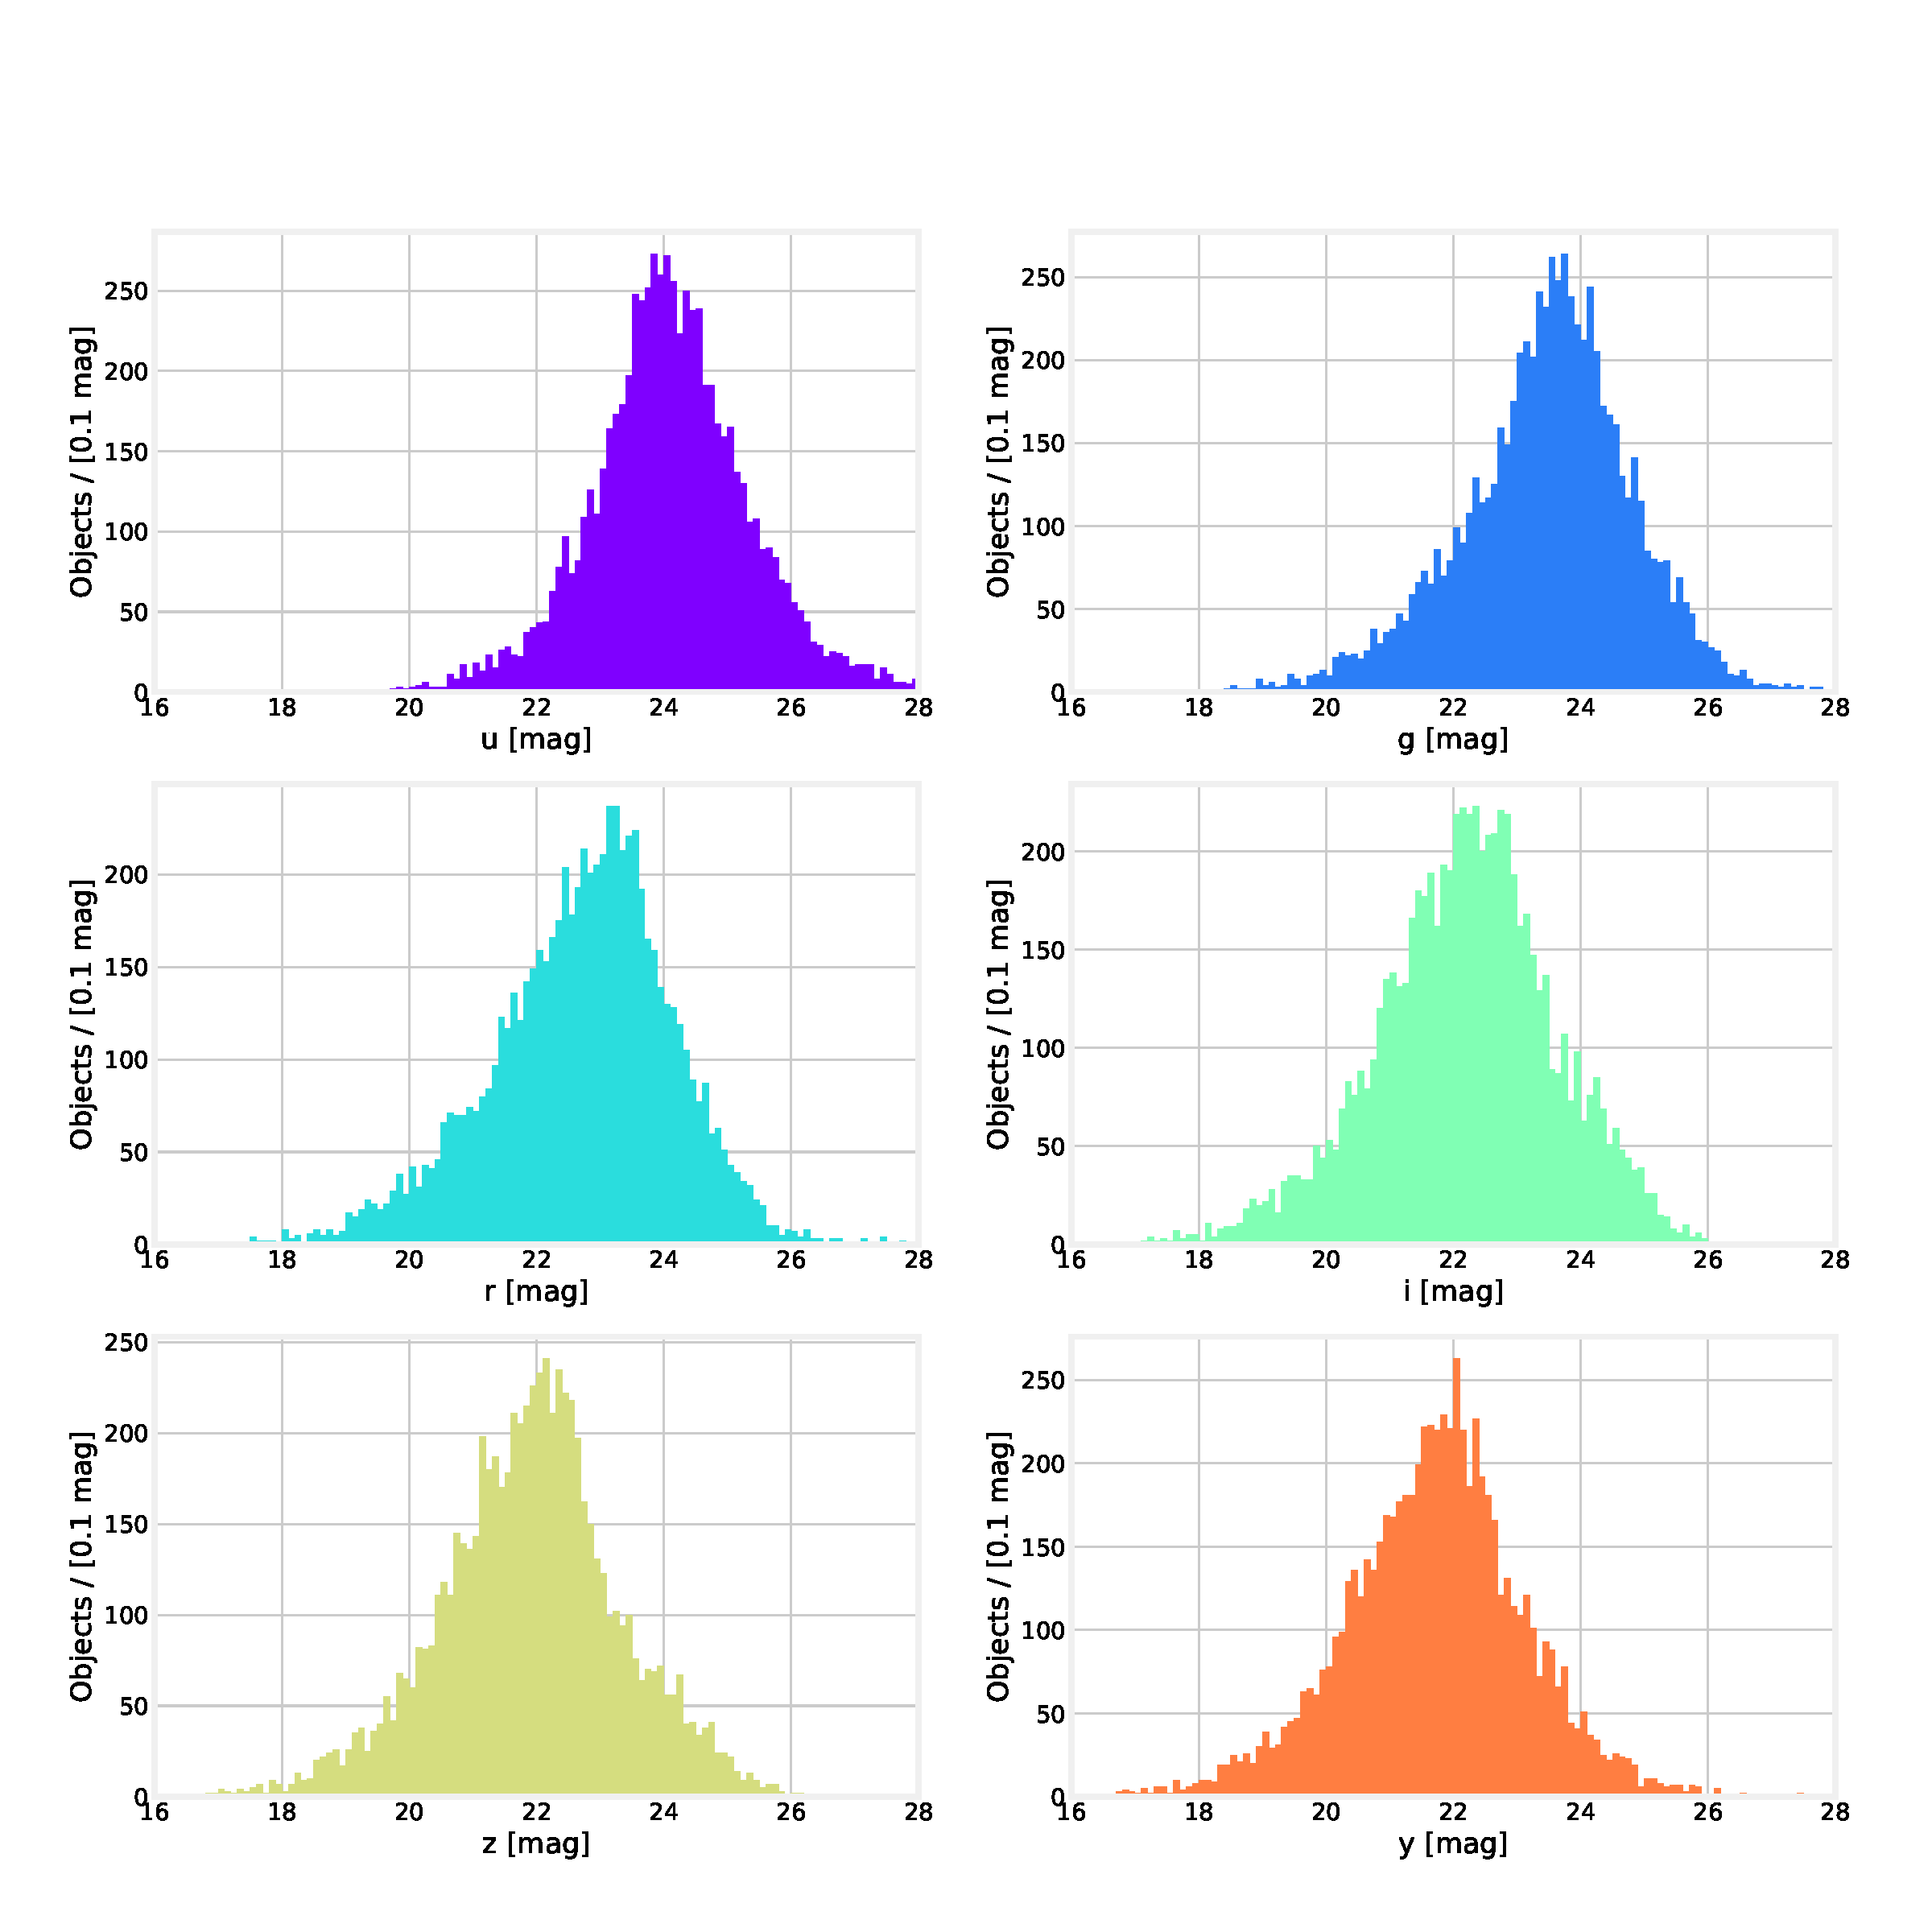
\includegraphics[width=\linewidth]{figures/mags.pdf}
    \caption{AB magntidues of objects passing the ``gold'' selection in each of the six rubin filter bands.} 
    \label{fig:dp_mags}
\end{figure*}

\begin{figure*}
    \centering
    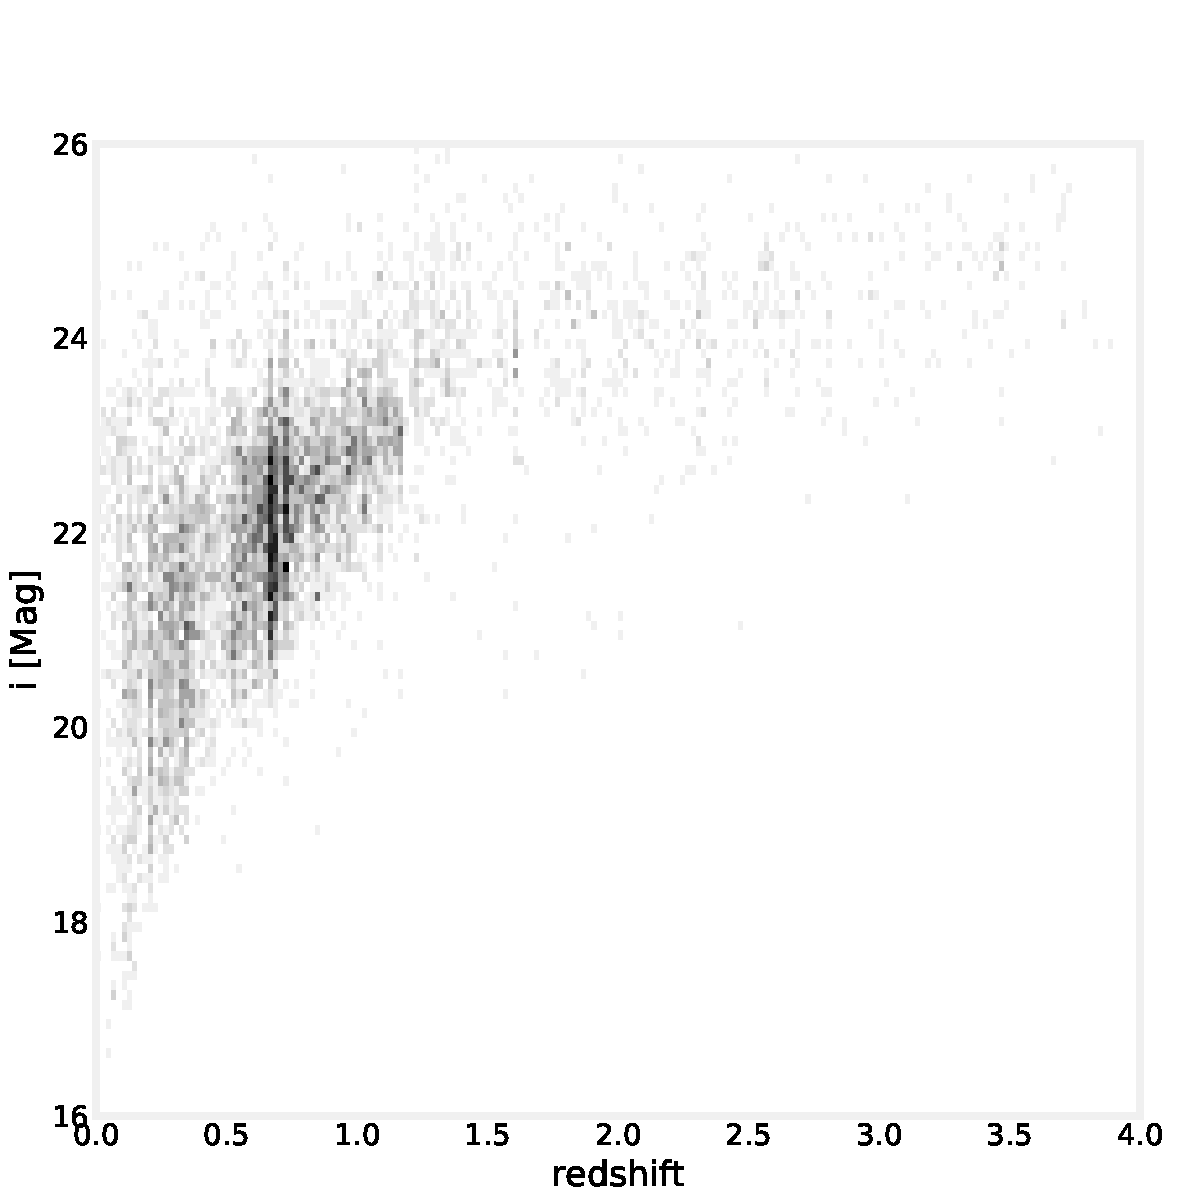
\includegraphics[width=\linewidth]{figures/mag_i_v_redshift.pdf}
    \caption{I-band magntidue versus redshift for all objects in the ``test'' dataset.}
    \label{fig:dp_mag_i_v_redshift}
\end{figure*}

\begin{figure*}
    \centering
    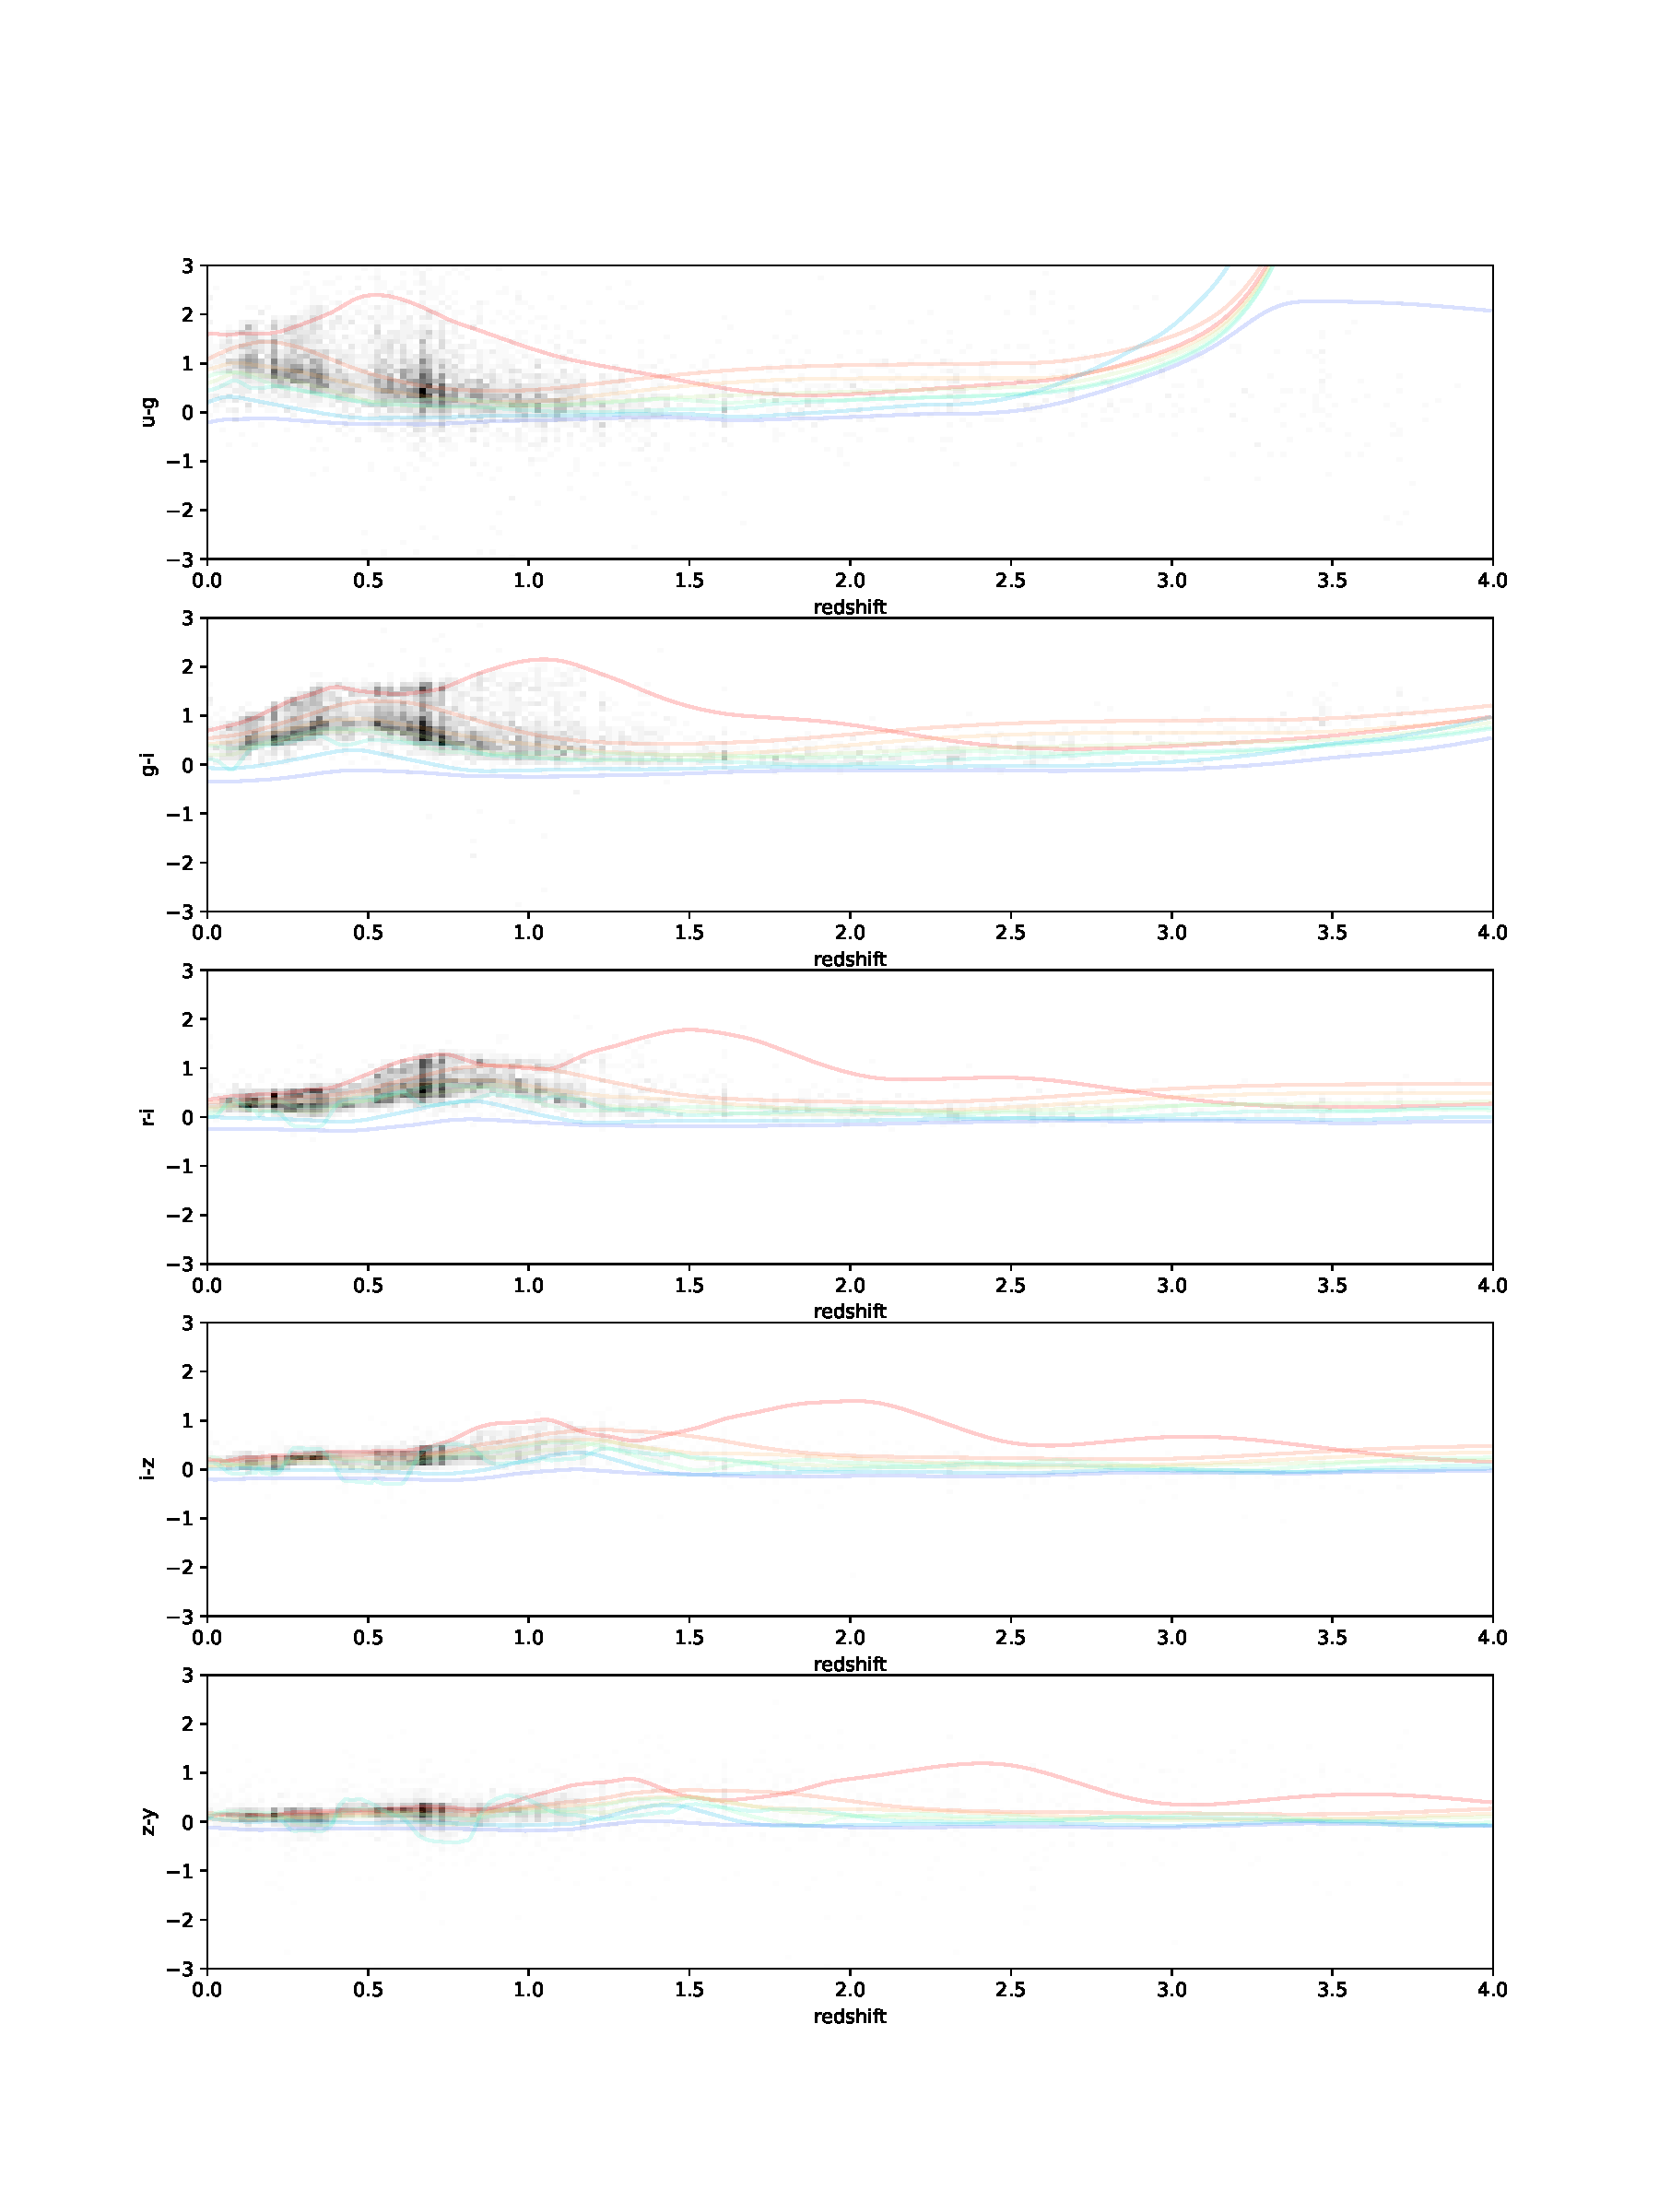
\includegraphics[width=\linewidth]{figures/color_v_redshift.pdf}
    \caption{``Adjacent band colors'', i.e., $u-g$, $g-r$, $r-i$, $i-z$, $z-y$, versus redshift for all objects in the ``test'' dataset.}
    \label{fig:dp_color_v_redshift}
\end{figure*}


\begin{figure*}
    \centering
    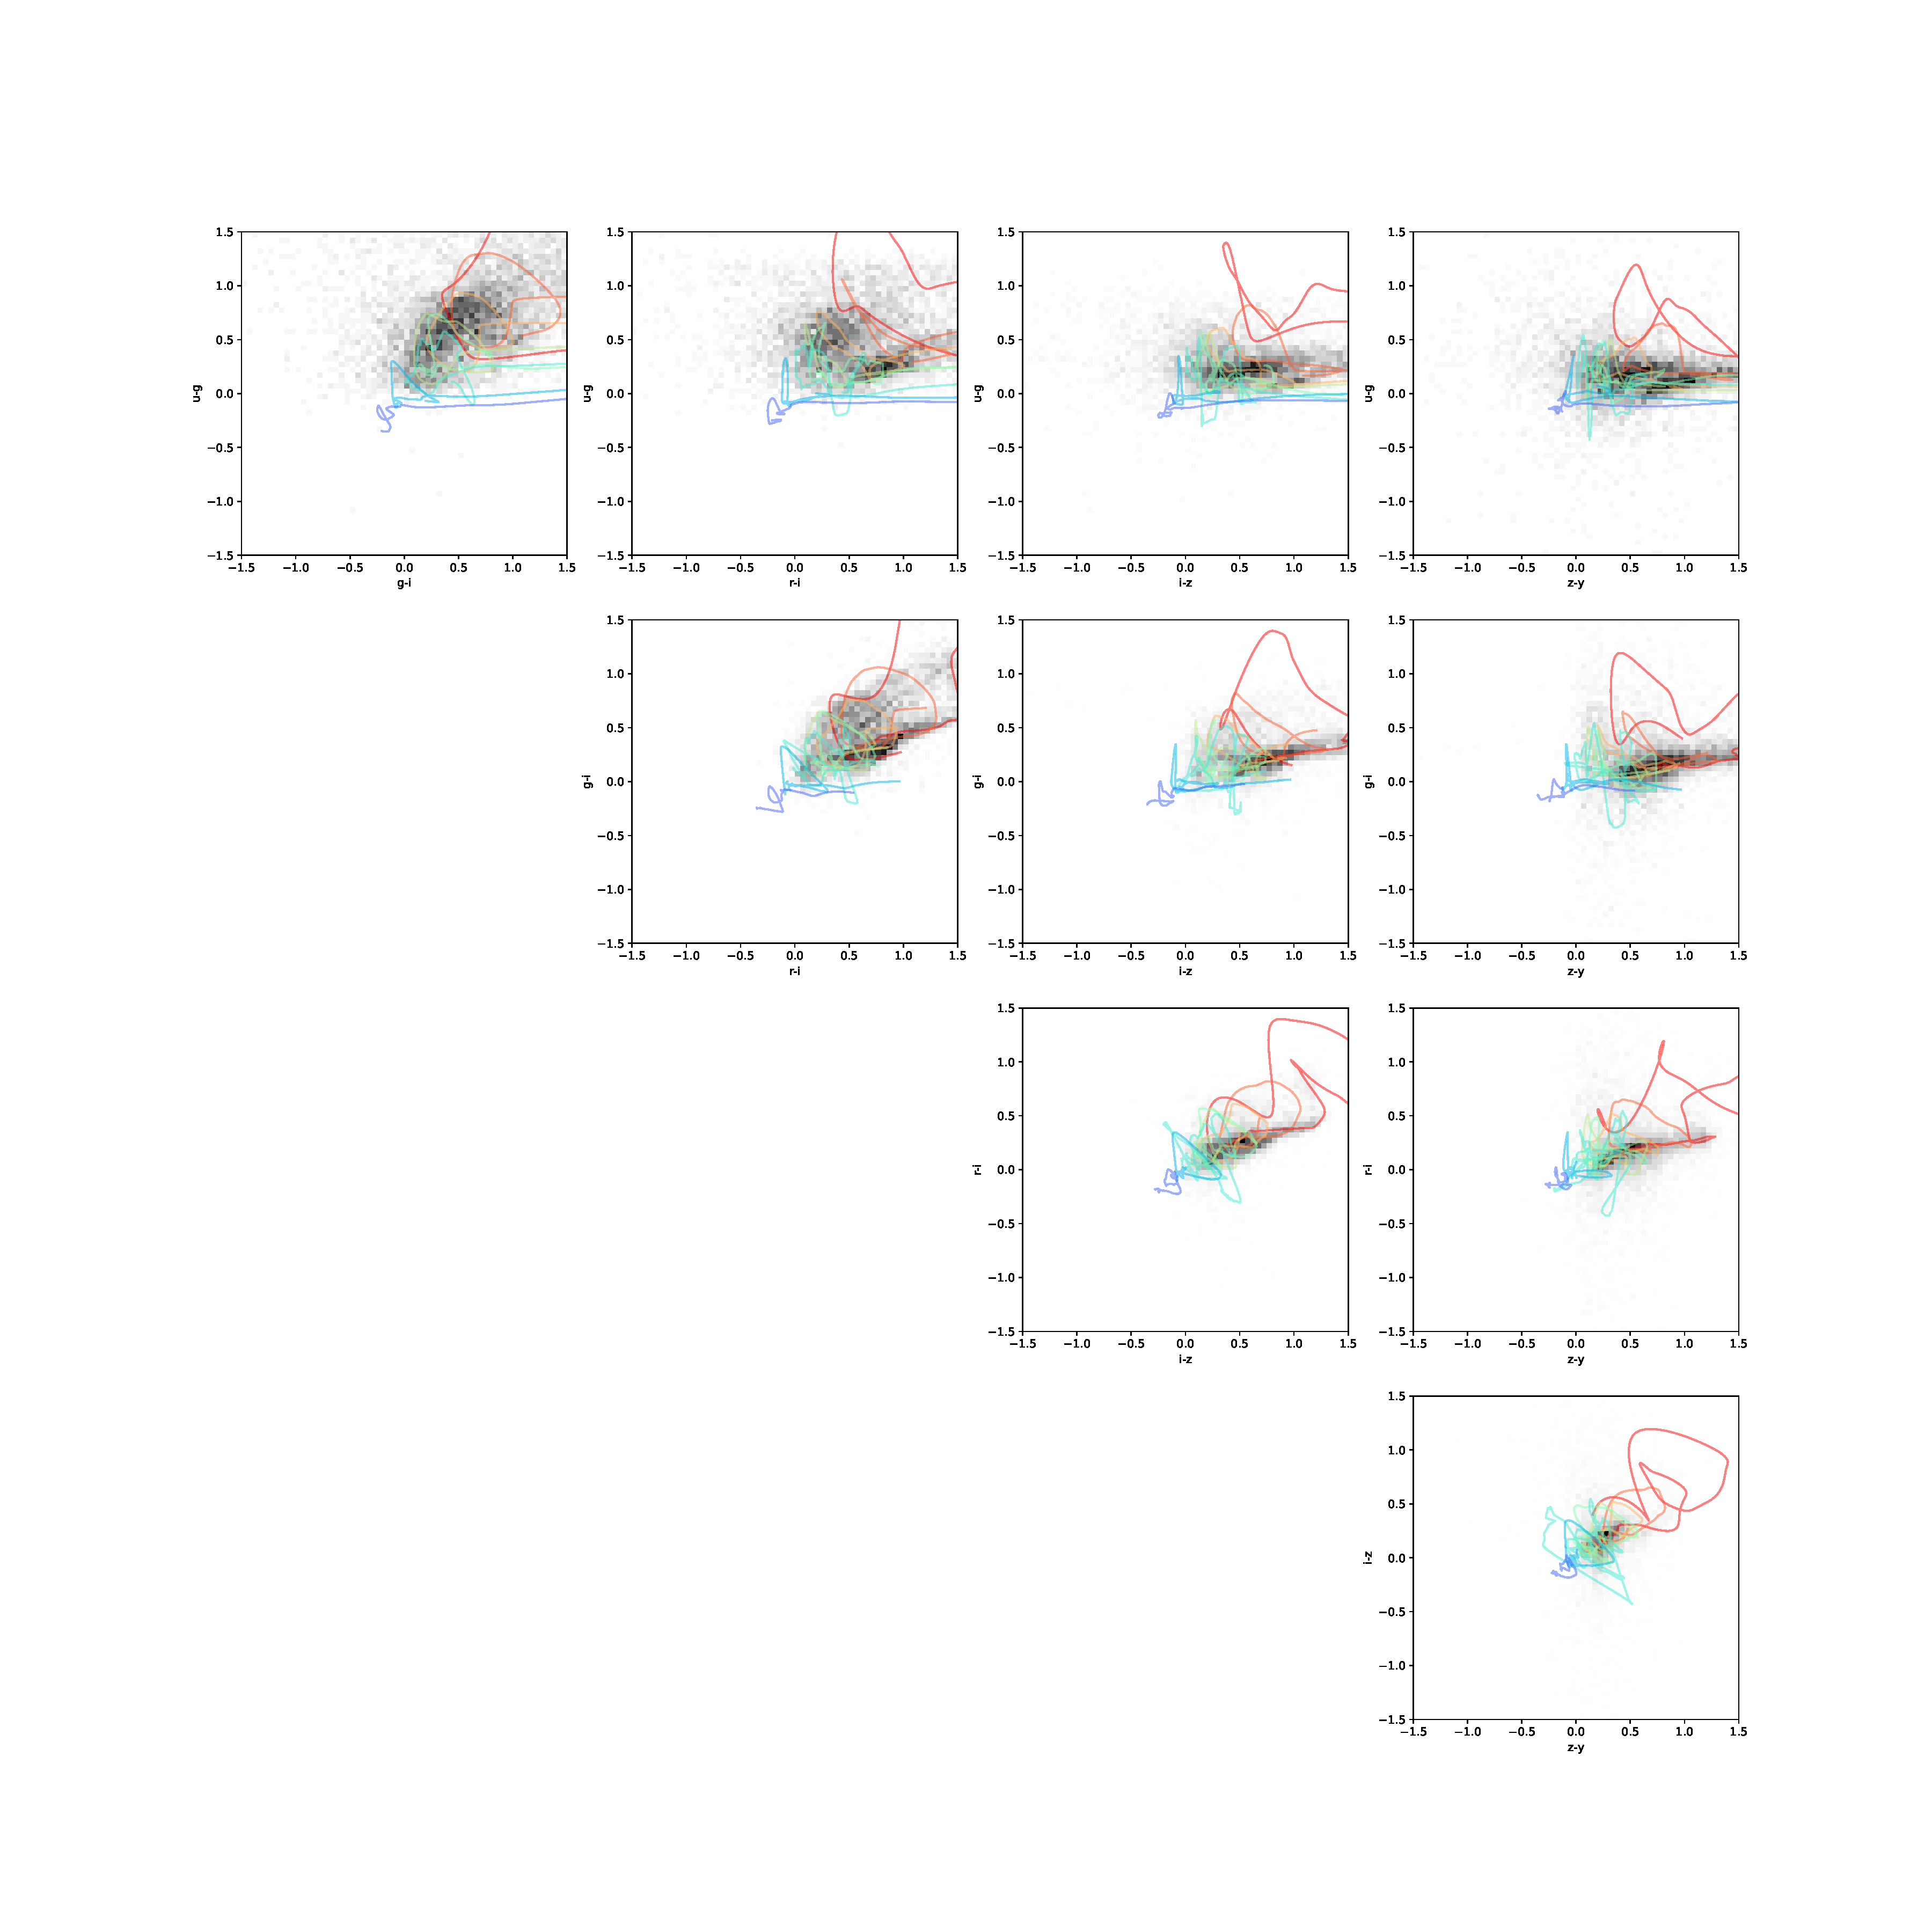
\includegraphics[width=\linewidth]{figures/color_v_color.pdf}
    \caption{Color-color correlations for the ``adjacent band colors'', for all objects in the ``test'' dataset.}
    \label{fig:dp_color_v_color}
\end{figure*}

\pagebreak


\subsection{Spectroscopic redshift reference sample}
\label{sec:data:reference}


\subsubsection{Euclid spectroscopic redshift dataset}
\label{sec:data:euclid}

\begin{figure*}
    \centering
    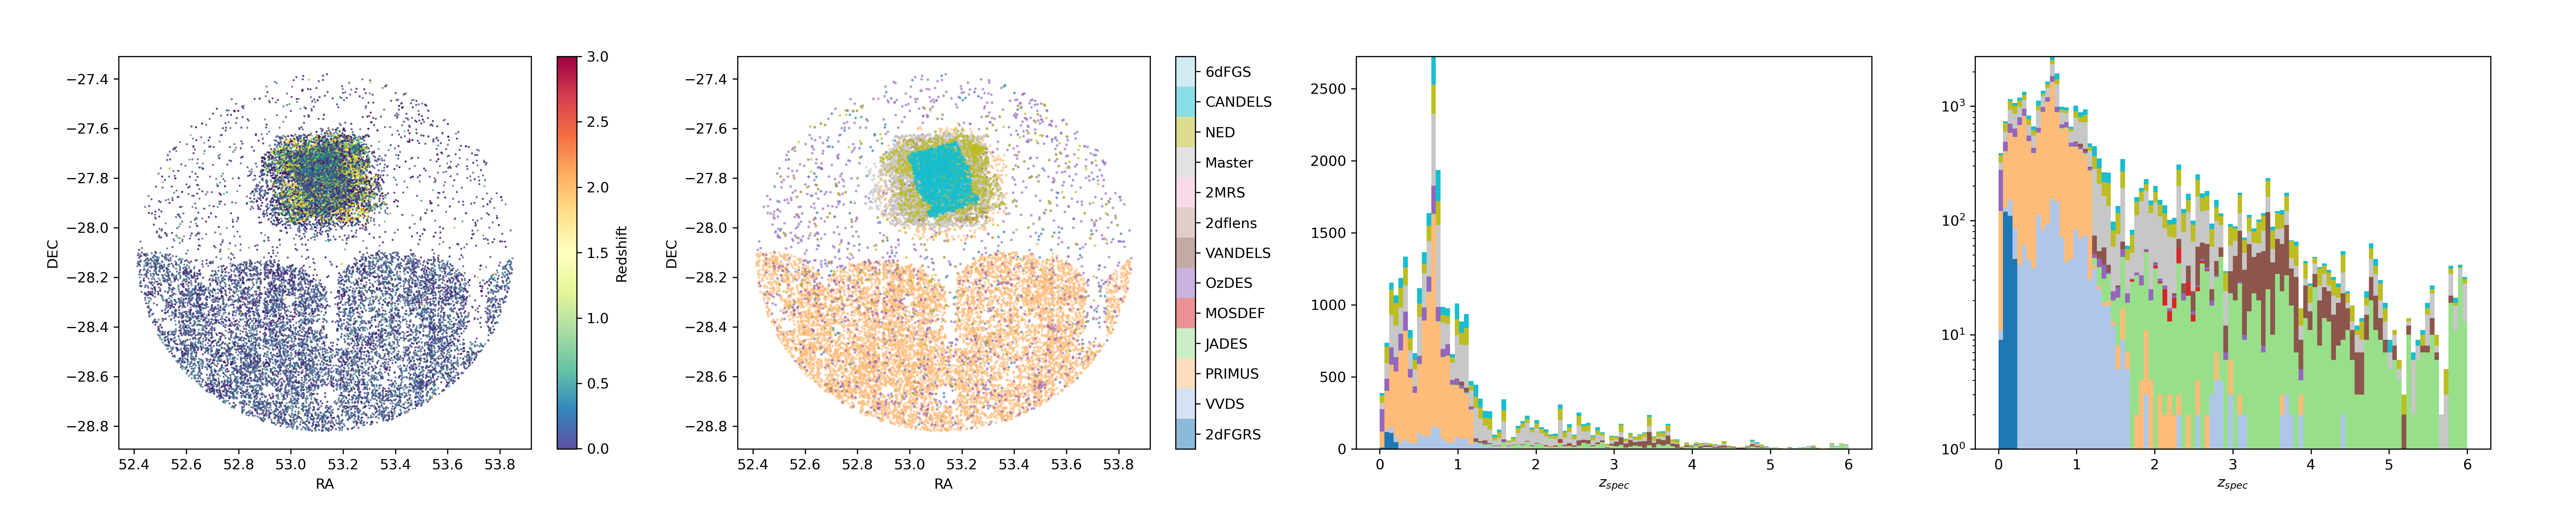
\includegraphics[width=1.0\linewidth]{figures/training_set_info.png}
    \caption{Training set in the ECDFS field. Panel 1: Scatter plot of the ECDFS reference catalog color coded by redshift. Panel 2: scatter plot of the ECDFS reference catalog color coded by the survey name. Panel 3 and Panel 4: redshift distribution with y-axis in linear and log scale. }
    \label{fig:enter-label}
\end{figure*}

\subsubsection{DESI Data Release 1 spectroscopic redshift dataset}
\label{sec:data:desi}


\section{Methodology}
\label{sec:method:0}

\begin{table*}
\centering
\begin{tabular}{lll}
 \hline
    Algorithm name  & Home package & Reference\\
 \hline
 \hline
 \multicolumn{3}{c}{Project Supported} \\ 
  \code{BPZ} & \href{https://github.com/LSSTDESC/rail_bpz}{\code{rail-bpz}} & \citet{Benitez:2000}\\
 \code{KNN} & \href{https://github.com/LSSTDESC/rail_sklearn}{\code{rail-sklearn}} & RAIL Paper\\
 \multicolumn{3}{c}{Commuity Supported} \\   
 \code{CMNN} & \href{https://github.com/LSSTDESC/rail_cmnn}{\code{rail-cmnn}} & \citet{Graham:2018}\\
 \code{DNF} & \href{https://github.com/LSSTDESC/rail_dnf}{\code{rail-dnf}} & \citet{2016MNRAS.459.3078D}\\
 \code{FlexZBoost}  & \href{https://github.com/LSSTDESC/rail_flexzboost}{\code{rail-flexzboost}} & \citet{Izbicki:2017}\\
 \code{GPz} & \href{https://github.com/LSSTDESC/rail_gpz_v1}{\code{rail-gpz-v1}} & \citet{Almosallam:2016}\\
 \code{LePHARE} & \href{https://github.com/LSSTDESC/rail_lephare}{\code{rail-lephare}} & \citet{1999MNRAS.310..540A}\\
 \code{TPZ} & \href{https://github.com/LSSTDESC/rail_tpz}{\code{rail-tpz}} & \citet{Carrasco-Kind:2013}\\
 \hline
\end{tabular}
\caption{
Summary of the pre-wrapped estimators/summarizers/classifiers described in Sec.~\ref{sec:est}.}
\label{tab:alg}
\end{table*}

We used the RAIL (Redshift Assessment Infrastructure Layers) software package as the core tool for training, evaluating, and applying photometric redshift estimation models.   We also used RAIL to evaluate of the model performance through a suite of diagnostic metrics, including redshift bias, scatter (e.g., normalized median absolute deviation), and catastrophic outlier rate and to make diagnostic plots of the algoriths performance.

The photo-z models were trained using the spectroscopic datasets that were matched to DP1 photometric sources as described in Sec.\ref{sec:data:reference}, serving as labeled examples with known redshifts.   Specifically we use the \texttt{rail\_project} package (see \ref{sec:method:rail_project} to run RAIL's ``pz'' pipeline, found \href{https://github.com/LSSTDESC/rail_pipelines/blob/main/src/rail/pipelines/estimation/pz_all.py}{here}, consisting of ``Inform'' or training the models on the ``training'' dataset , and used those models in ``Estimation'' and ``Evaluation'' stages on the reserved ``test'' dataset to evalutate the algorithm performance.  We also used \texttt{rail\_project}  to run RAIL'z ``estimate'' pipeline, found \href{https://github.com/LSSTDESC/rail_pipelines/blob/main/src/rail/pipelines/estimation/estimate_all.py}{here}, to run the photometric redshift estimation on the entire DP1 data set.

We used this methodology to evaluate all the algorithms listed in Tab.~\ref{tab:alg}.  Note that the \code{KNN} and \code{BPZ} algorithms will be supported by the project data-management team, while the others will be supported by the wider community, the RAIL development team and DESC collaboration.


\subsection{Template fitting based estimators}
\label{sec:method:template}

RAIL’s template-based fitting algorithms are designed to estimate photometric redshifts by comparing observed galaxy photometry to a set of predefined theoretical or empirical galaxy templates.  These templates represent different galaxy spectral energy distributions (SEDs) across various redshifts, capturing the expected variation in observed colors due to redshifted light.  When applied to a photometric dataset, the algorithm fits the observed galaxy’s multi-band photometry to these templates by minimizing the difference between the observed and model fluxes in each band, typically using a chi-squared or likelihood-based fitting procedure.  This process allows the algorithm to determine the most likely redshift for a given galaxy by identifying the template that best matches its observed color signature.


\subsection{Machine learning based estimators}
\label{sec:method:machine_learning}



\subsection{Analysis framework and bookkeeping software}
\label{sec:method:rail_project}


The \texttt{rail\_projects} software package within the RAIL ecosystem provides an essential framework for managing and organizing large-scale photometric redshift estimation workflows.  It acts as a project management and book-keeping tool that helps users streamline their research, especially when working with complex or large datasets, like those associated with the Rubin DP1 data.  The primary focus of \texttt{rail\_project} is to offer a systematic way to track different stages of data processing, model training, evaluation, and results across multiple experiments, ensuring that all tasks are well-documented and reproducible.

Additionally, \texttt{rail\_projects} facilitates the management of large datasets by organizing data into structured directories and providing interfaces for batch processing.  It allows users to scale up their work to handle not only large catalogs of objects but also multiple datasets and redshift estimation tasks.  The package ensures that datasets and models are kept in sync across various stages, from raw input data to intermediate results to final outputs.  This approach minimizes data mismanagement or errors during processing and enhances reproducibility, which is critical when dealing with large, complex scientific datasets like those produced by the Rubin Observatory.


\section{Data products}
\label{sec:products:0}

In the course of this work, we generated several data products, including redshift estimates and a variety of others that can be use to reproduce those estimates and to facilitate thorough evaluation of the algorithm performance.  These products include: configuration files, see Sec.\ref{sec: products:configuration}, ancillary inputs, see Sec.\ref{sec: products: algo_files}, trained models, see Sec.\ref{sec: products:models}, redshift estimatesm, see Sec.\ref{sec: products:qp_ensembles}, summary statistics,  see Sec.\ref{sec: products: summary_statistics}, and performance monitoring plots, see Sec.\ref{sec: products: peformance_plots}, all of which are essential for understanding the quality of the photometric redshift estimates and for refining the algorithms.   Together, these data products provide a comprehensive framework for conducting, managing, and evaluating photometric redshift estimation workflows in Rubin DP1.  They ensure that the process is not only scientifically rigorous but also organized and reproducible, enabling effective collaboration and ongoing refinement of photometric redshift techniques.


\subsection{Configuration files}
\label{sec: products:configuration}

The configuration files, collected \href{https://github.com/lsstdesc/rail_project_config}{in the GitHub ``rail\_project\_config''} repository, provide the necessary parameters and settings to control the various stages of the redshift estimation process, are a key element of \texttt{rail\_projects} workflow.  These files typically include specifications for the photometric bands used (e.g., g, r, i, z), the algorithm choices (e.g., template fitting or machine learning methods), details about data preprocessing, such as feature normalization and handling of missing data.  These configuration files also specify the training and validation dataset splits, hyperparameters for machine learning models, and paths for input/output data.  These files are essential for ensuring reproducibility and for sharing the exact settings used in different redshift estimation runs, enabling other researchers to replicate or extend the analysis. 

\subsection{Ancillary input files}
\label{sec: products:algo_files}

In addition to the configuraiton files, we require ancillary inputs such as filter definitions and galaxy spectral energy distribution (SED) template.  Filter definitions specify the characteristics of the observational filters used in Rubin DP1, including the filter transmission curves and their corresponding central wavelengths.  These definitions are essential for converting the raw photometric measurements into meaningful colors and for matching the observed data to theoretical or empirical galaxy templates.  Galaxy SED templates are collections of theoretical or observed spectra for galaxies at different redshifts and with different properties (e.g., galaxy type, age, star formation history).  These templates are used by template-fitting algorithms to model the expected galaxy colors as a function of redshift, allowing for the estimation of photometric redshifts by comparing observed colors to those predicted by the templates.   \eac{Sam, can you add something here?}


\subsection{Estimator data models}
\label{sec: products:models}

After training, the trained models for each photometric redshift estimation algorithm are stored as serialized files, either in Pickle (for Python-based models) or YAML (for model configurations) format.  These models encapsulate the learned relationships between photometric features (such as magnitudes and colors) and redshift values, allowing them to be applied to new data for redshift estimation.  These files store the final state of the model, including the weights, biases, and other learned parameters for machine learning models.  In the case of template-fitting methods, the corresponding model files may include the template sets and the fitting parameters.  The Pickle or YAML format ensures that the models can be easily loaded, applied to new datasets, and evaluated in future experiments.


\subsection{Redshift estiates stored as QP ensembles}
\label{sec: products:qp_ensembles}

The pre-object redshift estimates generated by the photometric redshift algorithms are stored in "qp" files.  These files serve as containers for storing the redshift predictions for each object in the dataset before any detailed statistical analysis or final reporting.  In the "qp" files, each galaxy’s redshift estimate is stored in a format that is compatible with the algorithm providing the estimate.  These files are designed to be lightweight and easy to query, allowing users to quickly retrieve the redshift estimates for individual objects.  The structure of "qp" files is optimized for efficient access and data retrieval, making it easier for users to process and analyze large numbers of photometric redshift estimates across large datasets like Rubin DP1.

\eac{Do we want a few lines about how to use qp?}


\subsection{Per-Object Summary Statistics}
\label{sec: products:summary_statistics}

In addition to the raw redshift estimates, the "qp" files also store per-object summary statistics in the form of an ancillary table.  These statistics include crucial information about the quality and reliability of each photometric redshift estimate, such as the uncertainty in the redshift prediction (e.g., the confidence interval or standard deviation or, the likelihood score (in the case of probabilistic models).   This table will eventually includes flags for identifying objects with low-confidence estimates or those that may be outliers.  These summary statistics are important for evaluating the overall performance of the redshift estimation algorithms on an object-by-object basis and are often used to filter out low-quality or problematic redshift estimates before conducting larger statistical analyses.

\eac{TQ, can you add table of summary stats and clarify about outlier rejection in compute said summary stats.}



\subsection{Performance Monitoring Plots}
\label{sec:products:peformance_plots}

Finally, we produced standardized performance monitoring plots as part of the photometric redshift workflow.  These plots provide visual representations of the model's performance, allowing users to assess how well the redshift estimates align with the true redshifts from the spectroscopic training data.  Common plots include:

\begin{itemize}
\item{Input dataset characterization plots, as shown in Sec.~\ref{sec:data:dp1:properties}.}
\item{Scatter plots to visualize the relationship between the predicted and true redshifts, highlighting any systematic biases or non-linearities.}
\item{Redshift comparison plots (e.g., the redshift residuals or bias vs.  true redshift), which show, e.g., the difference between the predicted and true redshifts as a function of redshift or object magntidue.}
\end{itemize}

Examples of the two latter types of plots for the \texttt{BPZ} and \texttt{KNN} algorithms are shown in Sec.~\ref{sec:performance:0}



\section{Data Distribution}
\label{sec:distribution:0}

To support both the Rubin community and the DESC, we will distrbute these data products in at least 3 different ways:
\begin{enumerate}
\item{Via the Rubin Data Butler.}
\item{Via the LIneA Photo-Z Server.}
\item{Directly as files at the USDF and NERSC.}
\end{enumerate}

\subsection{Distribution via the Rubin Data Butler}
\label{sec:distribution:butler}


\subsection{Distribution via the LIneA Photo-Z Server}
\label{sec:distribution:linea}


\subsection{Distribution as files at USDF and NERSC}
\label{sec:distribution:files}



\section{Performance}
\label{sec:performance:0}

We evaluated all seven of the algorithms listed in Tab.~\ref{tab:alg} for both scientific and technical performance.   Specifically 

\subsection{Redshift estimator performance}
\label{sec: performance:pz}


\begin{figure*}
    \centering
    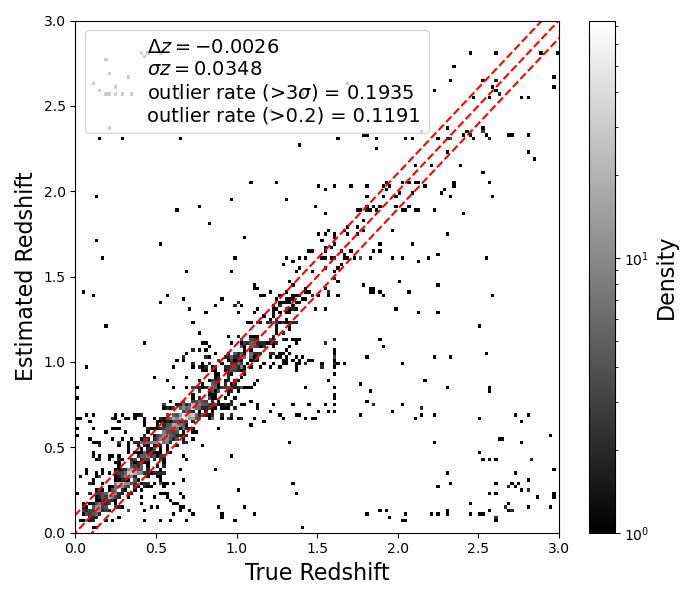
\includegraphics[width=0.45\linewidth]{figures/zestimate_v_ztrue_hist2d_knn.png}
    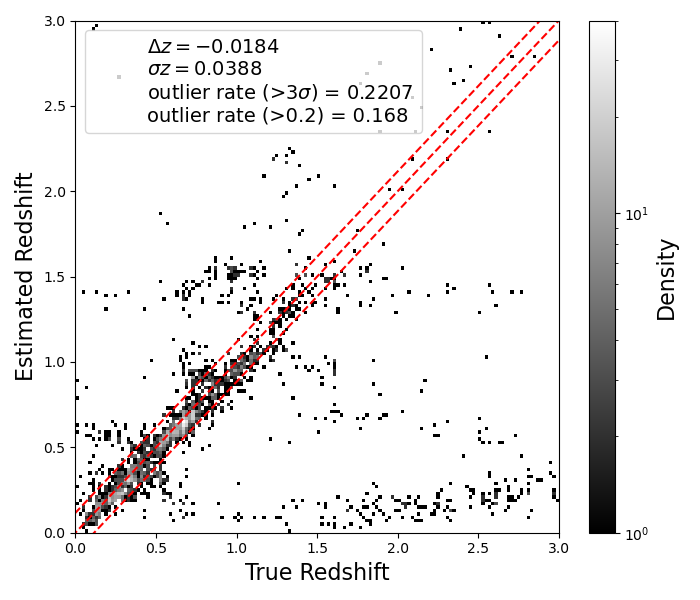
\includegraphics[width=0.45\linewidth]{figures/zestimate_v_ztrue_hist2d_bpz.png} \\
    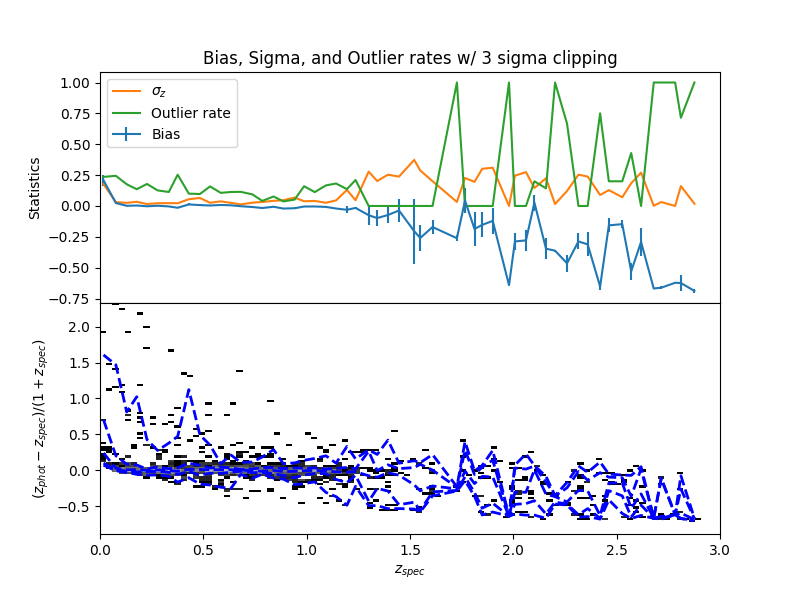
\includegraphics[width=0.45\linewidth]{figures/biweight_stats_v_redshift_knn.png}
    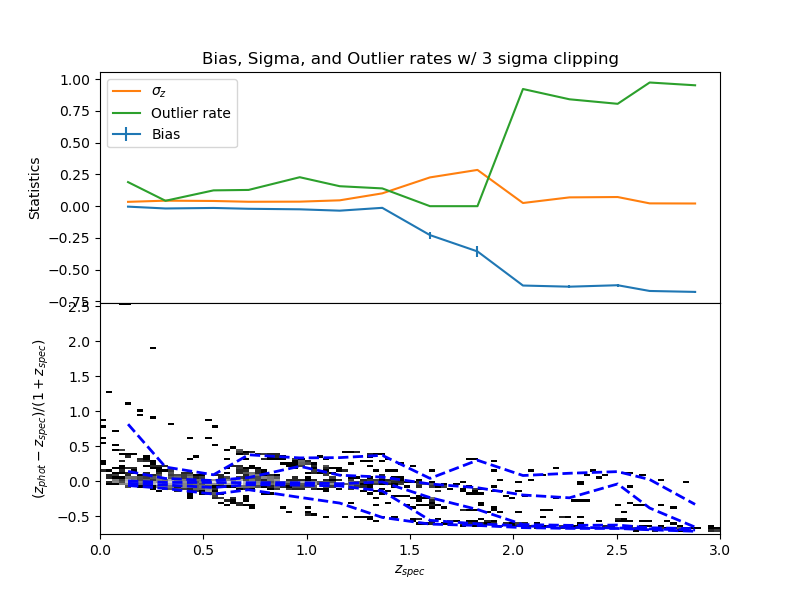
\includegraphics[width=0.45\linewidth]{figures/biweight_stats_v_redshift_bpz.png} \\
    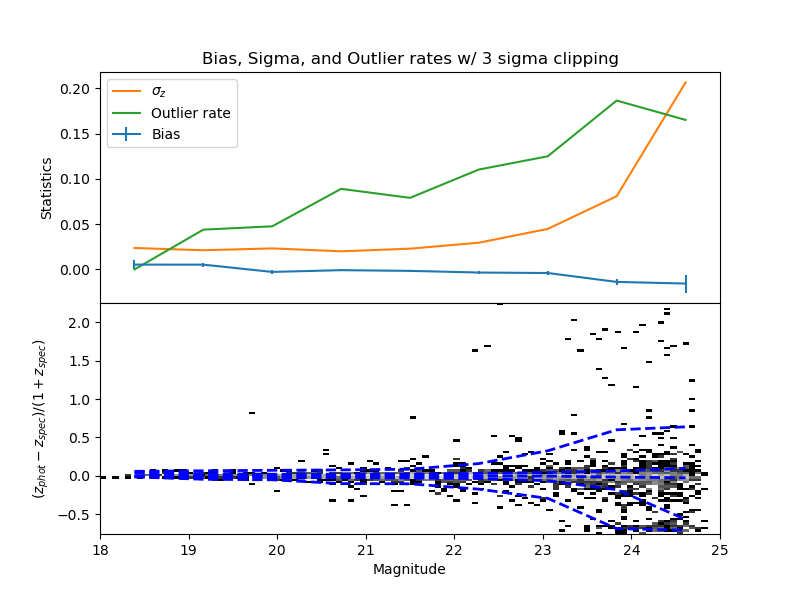
\includegraphics[width=0.45\linewidth]{figures/biweight_stats_v_mag_knn.png}
    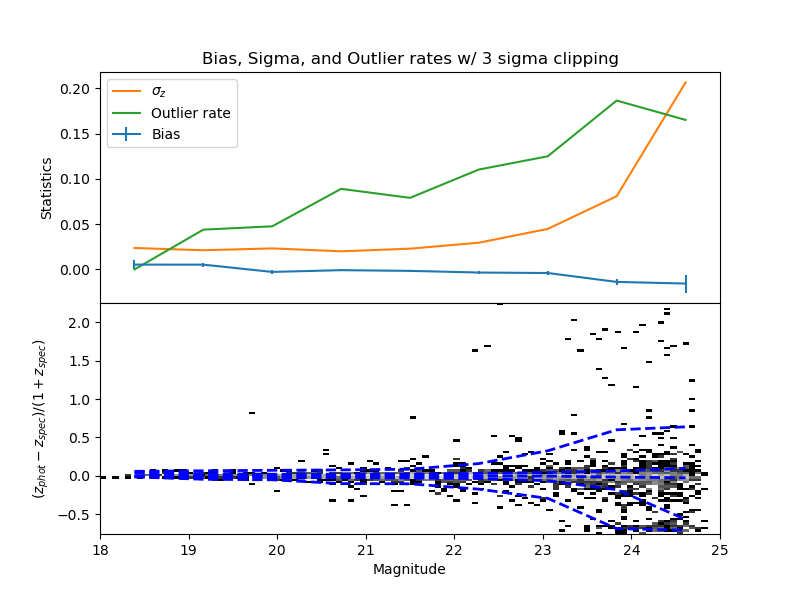
\includegraphics[width=0.45\linewidth]{figures/biweight_stats_v_mag_knn.png}    
    \caption{Estimator performance on the ``gold'' (six-band') dataset.  Top row: photometric point estimate of the redshift versus spectroscopic redshift for \code{KNN} (left) and \code{bpz} (right).   Middle row: performance metrics, (width and bias of residual, and outlier rate) versus spectroscopic redshift.    Bottow row, performance metrics versus i-band magntidue.}
    \label{fig:perf_gold}
\end{figure*}

\begin{figure*}
    \centering
    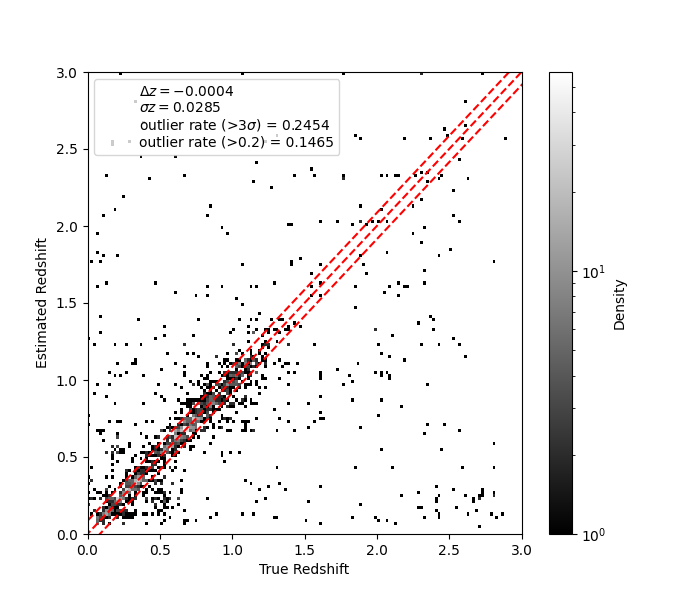
\includegraphics[width=0.45\linewidth]{figures/zestimate_v_ztrue_hist2d_knn_4.png}
    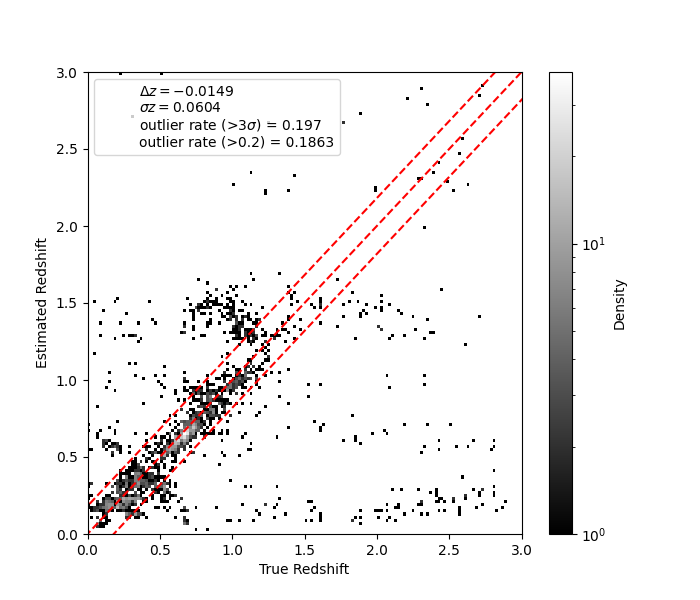
\includegraphics[width=0.45\linewidth]{figures/zestimate_v_ztrue_hist2d_bpz_4.png} \\
    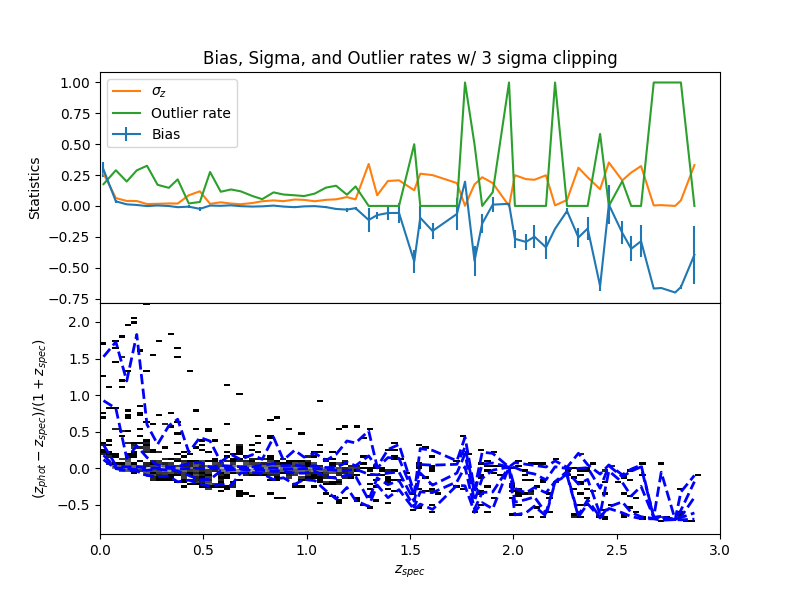
\includegraphics[width=0.45\linewidth]{figures/biweight_stats_v_redshift_knn_4.png}
    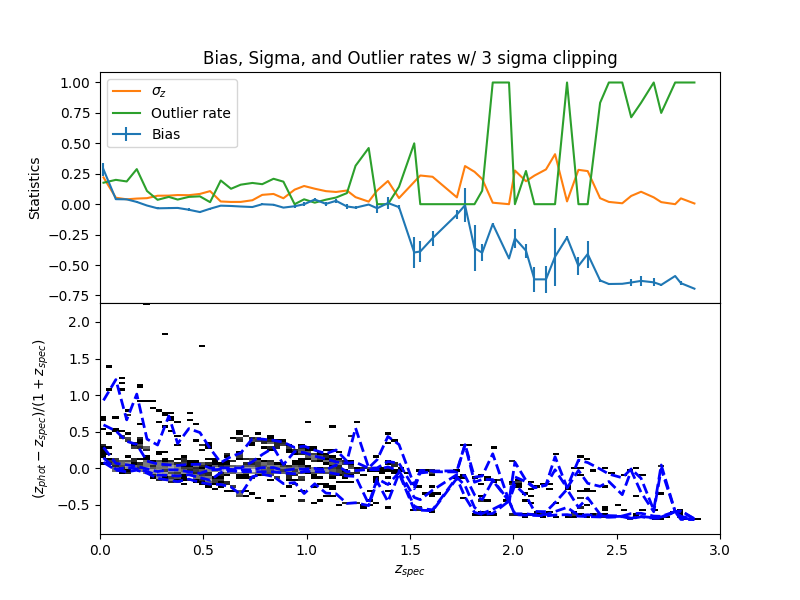
\includegraphics[width=0.45\linewidth]{figures/biweight_stats_v_redshift_bpz_4.png} \\
    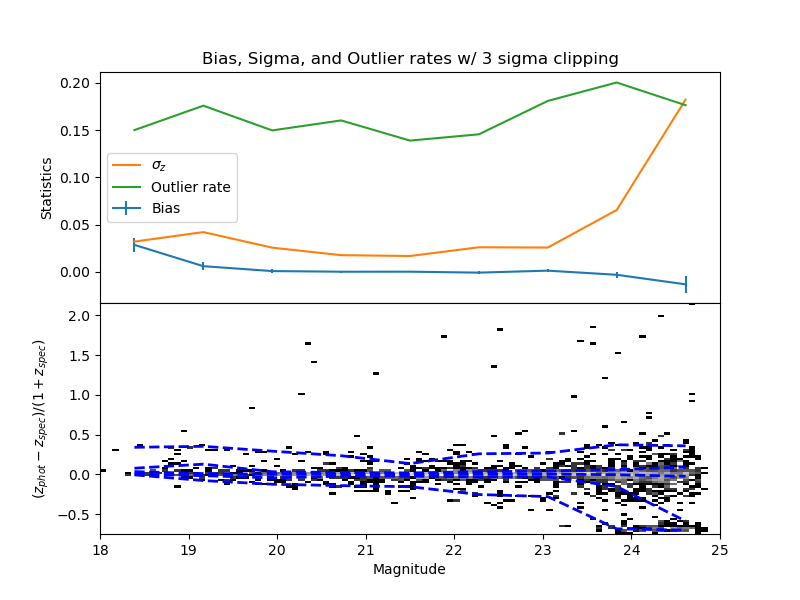
\includegraphics[width=0.45\linewidth]{figures/biweight_stats_v_mag_knn_4.png}
    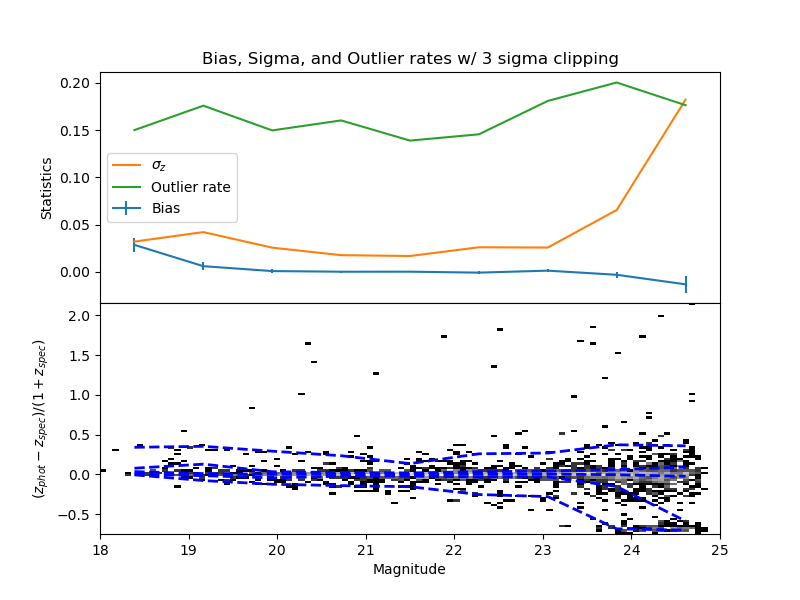
\includegraphics[width=0.45\linewidth]{figures/biweight_stats_v_mag_knn_4.png}    
    \caption{Estimator performance on the ``gold\_4\_band'' (four-band') dataset.  Top row: photometric point estimate of the redshift versus spectroscopic redshift for \code{KNN} (left) and \code{bpz} (right).   Middle row: performance metrics, (width and bias of residual, and outlier rate) versus spectroscopic redshift.    Bottow row, performance metrics versus i-band magntidue.}
    \label{fig:perf_gold_4_band}
\end{figure*}


\subsubsection{Redshift estimation quality flags}
\label{sec: performance:pz}



\subsection{Technical performacne}
\label{sec: performance:technical}

Tab.~\ref{tab:tech_perf} shows compute times and files sizes for both the training and estimation phases of the analysis.    The metrics from the training phase were taken from running the algorithn ``Inform'' states on USDF on the ``training'' dataset of ~13,000 objects.   

\begin{table*}
\centering
\begin{tabular}{lllll}
 \hline
  Algorithm name  & \multicolumn{2}{c}{Training}  &  \multicolumn{2}{c}{Estimation} \\
   & Time [s] & Model Size [MB] &  Speed [$\mu$ s / object] & Data Size [b / object] \\  
 \hline
 \hline
 \multicolumn{5}{c}{Project Supported} \\ 
  \code{BPZ} & & & & \\
 \code{KNN} & & & & \\
 \multicolumn{5}{c}{Community Supported} \\   
 \code{CMNN} & & & & \\
 \code{DNF} & & & & \\
 \code{FlexZBoost}  & & & & \\
 \code{GPz} & & & & \\
 \code{LePHARE} & & & & \\
 \code{TPZ} & & & & \\
 \hline
\end{tabular}
\caption{
  Algorithm compute times and files sizes.
}
\label{tab:tech_perf}
\end{table*}



\section{Summary and Conclusion}
\label{sec:summary:0}

We rocked it yo!


\pagebreak